\documentclass[11pt]{article}
\usepackage{graphics,graphicx}
%\usepackage[dvips]{graphics,graphicx}
\DeclareGraphicsExtensions{.ps,.jpg,.eps,.pdf,.png}
\usepackage{boxedminipage,amsmath,amsfonts}
\usepackage{url}
%\usepackage{secdot}
%\usepackage{natbib}
\usepackage{verbatim}
%\usepackage{moreverb}
\usepackage{enumerate}
\usepackage{makeidx}
\bibliographystyle{plain}
\makeindex


%%%%%
% some other macros
\newcommand{\figurepath}{./figures}
\newcommand{\bibpath}{/Users/kmartin/Documents/files/misc}
\newcommand{\figfiletype}{pdf}

%Brad Bell Macros

% Latex macros defined for all the CppAD documentation:
\newcommand{\T}{ {\rm T} }
\newcommand{\R}{ {\bf R} }
\newcommand{\C}{ {\bf C} }
\newcommand{\D}[2]{ \frac{\partial #1}{\partial #2} }
\newcommand{\DD}[3]{ \frac{\partial^2 #1}{\partial #2 \partial #3} }
\newcommand{\Dpow}[2]{ \frac{\partial^{#1}}{\partial  {#2}^{#1}} }
\newcommand{\dpow}[2]{ \frac{ {\rm d}^{#1}}{{\rm d}\, {#2}^{#1}} }

% Define the hangref environment used for the References list:
\newenvironment{hangref}
  {\begin{list}{}{\setlength{\itemsep}{4pt}
  \setlength{\parsep}{0pt}\setlength{\leftmargin}{+\parindent}
  \setlength{\itemindent}{-\parindent}}}{\end{list}}

% Set the page margins to 1 inch all around:
\marginparwidth 0pt\marginparsep 0pt \topskip 0pt\headsep
0pt\headheight 0pt \oddsidemargin 0pt\evensidemargin 0pt
\textwidth 6.5in \topmargin 0pt\textheight 9.0in
\newtheorem{theorem}{Theorem}


%%%%Added by Leo%%%%
\newcounter{Fig}
\renewcommand{\theFig}{\arabic{Fig}}
\newcommand{\Fig}[2]{\refstepcounter{Fig} \label{#1}
                     {\small\bf Figure \theFig.} {\small\sl #2 \par}}

\setcounter{topnumber}{3}
\renewcommand{\topfraction}{.9}
\setcounter{bottomnumber}{3}
\renewcommand{\bottomfraction}{.9}
\setcounter{totalnumber}{4}
\renewcommand{\textfraction}{.1}
\setlength{\floatsep}{.25in}
\setlength{\intextsep}{.25in}

\setlength{\fboxrule}{2\fboxrule} \setlength{\fboxsep}{3\fboxsep}

\newcommand{\Sa}{8pt}
\newcommand{\Sb}{0pt}

\renewcommand{\_}{{\char"5F}}
\renewcommand{\{}{{\char"7B}}
\renewcommand{\}}{{\char"7D}}
\renewcommand{\^}{{\char"0D}}

\let\accute= \'
\renewcommand{\'}{{\char"0D}}

\newcommand{\bfit}{\bfseries\itshape}

\newlength{\extopskip} \newlength{\exbottomskip}
\setlength{\exbottomskip}{1\baselineskip}
\addtolength{\exbottomskip}{-5.0pt}
\setlength{\extopskip}{1\exbottomskip}
\addtolength{\extopskip}{-1\parskip}

\newenvironment{Example}{\vspace{1\extopskip}\noindent\hspace*{2em}
                         \frenchspacing\small
                         \tt\begin{tabular}{@{}l@{}}}{
                         \end{tabular}\\[1\exbottomskip]}

\newcommand{\Titem}{\item[$\triangleright$]}
\newcommand{\Ditem}{\item[$\diamond$]}

\newenvironment{Itemize}{\begin{quote}\normalsize
   \baselineskip 20pt plus .3pt minus .1pt \begin{itemize}}
   {\end{itemize}\end{quote}}
   % Set path to folder containing figures
\newcommand{\FigureFolder}{figures}

\newif\ifknitro \knitrofalse    % change to \knitrotrue once we get knitro connected again
\newif\ifipopt  \ipopttrue      % change to \ipopttrue  once we get the build problems sorted out


% We use a number of URLs that point to software downloads. These locations are forever changing,
% and maintaining them is a nightmare. All the URLs are gathered here, so that we can at least
% get away with making changes only once...
\newcommand{\UrlAmpl}{http://www.ampl.com}
\newcommand{\UrlAmplSandia}{http://netlib.sandia.gov/ampl/}
\newcommand{\UrlAmplSolvers}{http://netlib.sandia.gov/cgi-bin/netlib/netlibfiles.tar?filename=netlib/ampl/solvers}
\newcommand{\UrlApacheFileupload}{http://jakarta.apache.org/commons/fileupload/}
\newcommand{\UrlBlas}{ftp://www.netlib.org/blas/blas.tgz}
\newcommand{\UrlBonmin}{http://projects.coin-or.org/Bonmin}
\newcommand{\UrlBuildtools}{http://projects.coin-or.org/BuildTools}
\newcommand{\UrlCbc}{http://projects.coin-or.org/Cbc}
\newcommand{\UrlCgl}{http://projects.coin-or.org/Cgl}
\newcommand{\UrlCl}{http://www.microsoft.com/express/download/\#webInstall}
\newcommand{\UrlClp}{http://projects.coin-or.org/Clp}
\newcommand{\UrlCoinConfig}{https://projects.coin-or.org/BuildTools/wiki/user-configure\#PreparingtheCompilation}
\newcommand{\UrlCoinConfigure}{http://projects.coin-or.org/BuildTools/wiki/user-configure\#CommandLineArgumentsforconfigure}
\newcommand{\UrlCoinCygwin}{http://projects.coin-or.org/BuildTools/wiki/current-issues}
\newcommand{\UrlCoinDownload}{http://projects.coin-or.org/BuildTools/wiki/user-download\#DownloadingtheSourceCode}
\newcommand{\UrlCoinNames}{https://projects.coin-or.org/CoinBinary/wiki/ArchiveNamingConventions}
\newcommand{\UrlCoinProjects}{http://www.coin-or.org/projects/}
\newcommand{\UrlCoinUtils}{http://projects.coin-or.org/CoinUtils}
\newcommand{\UrlCouenne}{http://projects.coin-or.org/Couenne}
\newcommand{\UrlCpl}{http://www.ibm.com/developerworks/library/os-cpl.html}
\newcommand{\UrlCplex}{http://www.ilog.com/products/cplex/}
\newcommand{\UrlCppad}{http://projects.coin-or.org/CppAD}
\newcommand{\UrlCygwinMake}{http://www.cmake.org/files/cygwin/make.exe}
\newcommand{\UrlCygwinSetup}{http://www.cygwin.com/setup.exe}
\newcommand{\UrlDoxygen}{http://www.doxygen.org}
\newcommand{\UrlDylp}{http://projects.coin-or.org/DyLP}
\newcommand{\UrlFToC}{http://www.netlib.org/f2c}
\newcommand{\UrlFToCBin}{http://www.netlib.org/f2c/mswin/}
\newcommand{\UrlFToCZip}{http://www.netlib.org/f2c/libf2c.zip}
\newcommand{\UrlGgs}{http://www.g95.org}
\newcommand{\UrlGamslinks}{https://projects.coin-or.org/svn/GAMSlinks/trunk}
\newcommand{\UrlGcc}{http://gcc.gnu.org}
\newcommand{\UrlGfortran}{http://gcc.gnu.org/fortran/}
\newcommand{\UrlGlpk}{http://www.gnu.org/software/glpk/}
\newcommand{\UrlGlpkDownload}{ftp://ftp.gnu.org/gnu/glpk/glpk-4.32.tar.gz}
\newcommand{\UrlHsl}{http://www.cse.scitech.ac.uk/nag/hsl/}
\newcommand{\UrlIpopt}{http://projects.coin-or.org/Ipopt}
\newcommand{\UrlIpoptDoc}{https://projects.coin-or.org/Ipopt/browser/stable/3.5/Ipopt/doc/documentation.pdf?format=raw}
\newcommand{\UrlIpoptDocxiii}{http://www.coin-or.org/Ipopt/documentation/node13.html}
\newcommand{\UrlKippFileupload}{http://gsbkip.chicagogsb.edu/os/fileupload.html}
\newcommand{\UrlKnitro}{http://www.ziena.com/}
\newcommand{\UrlKnitroMan}{http://www.ziena.com/docs/knitroman.pdf}
\newcommand{\UrlLapack}{ftp://www.netlib.org/lapack/lapack-lite-3.1.0.tgz}
\newcommand{\UrlMingw}{http://downloads.sourceforge.net/mingw/MSYS-1.0.11.exe?modtime=1079444447\&big\_mirror=1}
\newcommand{\UrlMsys}{http://sourceforge.net/project/showfiles.php?group\_id=2435}
\newcommand{\UrlMsysBinary}{http://downloads.sourceforge.net/mingw/bash-3.1-MSYS-1.0.11-1.tar.bz2?modtime=1195140582\&big\_mirror=1}
\newcommand{\UrlMsysAddIns}{http://sourceforge.net/project/showfiles.php?group\_id=2435\&package\_id=67879}
\newcommand{\UrlMsysBison}{bison-2.3-MSYS-1.0.11-1.tar.bz2}
\newcommand{\UrlMsysFlex}{flex-2.5.33-MSYS-1.0.11-1.tar.bz2}
\newcommand{\UrlMsysRegex}{regex-0.12-MSYS-1.0.11-1.tar.bz2}
\newcommand{\UrlNewticket}{http://projects.coin-or.org/OS/newticket}
\newcommand{\UrlNightlyBuild}{https://projects.coin-or.org/TestTools/wiki/NightlyBuildInAction}
\newcommand{\UrlOs}{http://www.optimizationservices.org}
\newcommand{\UrlOsBinaries}{http://www.coin-or.org/download/binary/OS/}
\newcommand{\UrlOsCommon}{https://projects.coin-or.org/svn/OS/branches/OScpp/OSCommon}
\newcommand{\UrlOsDoxygen}{http://www.coin-or.org/OS/doxydoc/html/index.html}
\newcommand{\UrlOsi}{http://projects.coin-or.org/Osi}
\newcommand{\UrlOsJava}{https://projects.coin-or.org/svn/OS/branches/OSjava}
\newcommand{\UrlOsRelease}{https://projects.coin-or.org/svn/OS/releases/1.1.1}
\newcommand{\UrlOsStable}{https://projects.coin-or.org/svn/OS/stable/1.1}
\newcommand{\UrlOsTarball}{http://www.coin-or.org/download/source/OS/}
\newcommand{\UrlOsWin}{https://projects.coin-or.org/CoinBinary/browser/binary/OS}
\newcommand{\UrlParinclinear}{http://www.coin-or.org/OS/parincLinear.osil}
\newcommand{\UrlSdk}{http://www.microsoft.com/downloads/details.aspx?FamilyID=E6E1C3DF-A74F-4207-8586-711EBE331CDC\&displaylang=en}
\newcommand{\UrlSvn}{http://subversion.tigris.org}
\newcommand{\UrlSymphony}{http://projects.coin-or.org/SYMPHONY}
\newcommand{\UrlTomcat}{http://tomcat.apache.org/}
\newcommand{\UrlTortoiseSvn}{http://tortoisesvn.tigris.org}
\newcommand{\UrlTrac}{http://projects.coin-or.org/OS}
\newcommand{\UrlUsingTrac}{http://www.coin-or.org/usingTrac.html}
\newcommand{\UrlVol}{http://projects.coin-or.org/Vol}
\newcommand{\UrlWget}{http://www.christopherlewis.com/WGet/WGetFiles.htm}
\newcommand{\UrlWgetBinary}{http://www.christopherlewis.com/WGet/wget-1.11.4b.zip}

% Current software versions
\newcommand{\GlpkVer}{4.32}
\newcommand{\OSstable}{2.0}
\newcommand{\OSrelease}{2.0.1}
\newcommand{\OStrunk}{2093}
\newcommand{\MsysVer}{1.0.11}
\newcommand{\MsysFile}{bash-3.1-MSYS-1.0.11}



\begin{document}

%Some cross-referencing index entries (to be expanded as needed)
\index{ASL|see{AMPL Solver Library (ASL)}}
\index{HSL|see{Harwell Subroutine Library (HSL)}}
\index{nl files|see{AMPL nl format}}
\index{Bonmin@{\tt Bonmin}|see{COIN-OR projects, {\tt Bonmin}}}
\index{BuildTools@{\tt BuildTools}|see{COIN-OR projects, {\tt BuildTools}}}
\index{Cbc@{\tt Cbc}|see{COIN-OR projects, {\tt Cbc}}}
\index{Cgl@{\tt Cgl}|see{COIN-OR projects, {\tt Cgl}}}
\index{Clp@{\tt Clp}|see{COIN-OR projects, {\tt Clp}}}
\index{Configuration Manager|see{Microsoft Visual Studio, Configuration Manager}}
\index{Couenne@{\tt Couenne}|see{COIN-OR projects, {\tt Couenne}}}
\index{CppAD@{\tt CppAD}|see{COIN-OR projects, {\tt CppAD}}}
\index{CoinUtils@{\tt CoinUtils}|see{COIN-OR projects, {\tt CoinUtils}}}
\index{Debug configuration|see{Microsoft Visual Studio, {\tt Debug} configuration}}
\index{DyLP@{\tt DyLP}|see{COIN-OR projects, {\tt DyLP}}}
\index{Ipopt@{\tt Ipopt}|see{COIN-OR projects, {\tt Ipopt}}}
\index{Osi@{\tt Osi}|see{COIN-OR projects, {\tt Osi}}}
\index{Release configuration|see{Microsoft Visual Studio, {\tt Release} configuration}}
\index{Release-plus configuration|see{Microsoft Visual Studio, {\tt Release-plus} configuration}}
\index{SYMPHONY@{\tt SYMPHONY}|see{COIN-OR projects, {\tt SYMPHONY}}}
\index{Vol@{\tt Vol}|see{COIN-OR projects, {\tt Vol}}}

\title{Using COIN-OR Solvers with Visual Studio}
\vskip 2in
\author{Horand Gassmann, Jun Ma,  and  Kipp Martin}
\maketitle

\begin{abstract}
This is for Windows users that want to run COIN-OR solvers directly from a file or a modeling language, or want to write applications with Visual Studio projects that use COIN-OR solvers. This download is plug-and-play it is not necessary to build any COIN-OR projects from source code.
\end{abstract}


\newpage
\tableofcontents
%\listoffigures
%\listoftables
\hyphenation{com-plex-Type}
\hyphenation{GAMS-links}



%\noindent\hrulefill
\newpage

\section{The Download}

\section{Calling COIN-OR Solvers with Model Instances}

In the {\tt bin} directory, the user will find the following solvers (see the project link for more information on the solvers):
\begin{itemize}
\item {\bf bonmin.exe} -- a solver for mixed-integer nonlinear programs-- see \url{https://projects.coin-or.org/Bonmin}

\item {\bf cbc.exe} --  a solver for mixed-integer linear programs --  see \url{https://projects.coin-or.org/Cbc}

\item {\bf clp.exe} -- a solver for linear programs  -- see \url{https://projects.coin-or.org/Clp}

\item {\bf couenne.exe} -- a global optimizer for mixed-integer nonlinear programs  -- see \url{https://projects.coin-or.org/Couenne}

\item {\bf ipopt.exe} -- an optimizer for continuous nonlinear programs -- see \url{https://projects.coin-or.org/Ipopt}

\item {\bf symphony.exe} -- a solver for mixed-integer linear programs -- see \url{https://projects.coin-or.org/SYMPHONY}
\end{itemize}

See the project pages for a more detail on each of the solvers and which optimization instance format they take.

For the convenience of the user, the bin directory also contains the {\bf OSSolverService.exe}.  This executable is linked to libraries for all of the above solvers, and can be used in lieu of any of them. One advantage of using the {\it OSSolverService.exe}  is its flexibility. You can call any of the above solvers with an instance in MPS, nl, or OSiL format.   In addition, the {\bf OSSolverService.exe} returns the solver solution in the OSrL XML format which is easily parsed. 


{\bf Solve a  linear program:}  using the  {\tt OSSolverService} .  At the command line,  connect ({\bf cd}) to the bin directory and execute the following:


\vfill
\begin{center}
To solve  a problem in OSiL XML format
\end{center}
\vfill

{\small
\begin{verbatim}
OSSolverService -osil ../../data/osilFiles/parincLinear.osil
\end{verbatim}

\vfill
\begin{center}
To solve a problem in AMPL nl format
\end{center}
\vfill

\begin{verbatim}
OSSolverService -nl ../../data/amplFiles/parinc.nl
\end{verbatim}

\vfill
\begin{center}
To solve a problem in MPS format
\end{center}
\vfill

\begin{verbatim}
OSSolverService -mps ../../data/mpsFiles/parinc.mps
\end{verbatim}
}%end small



The result is printed in XML format:


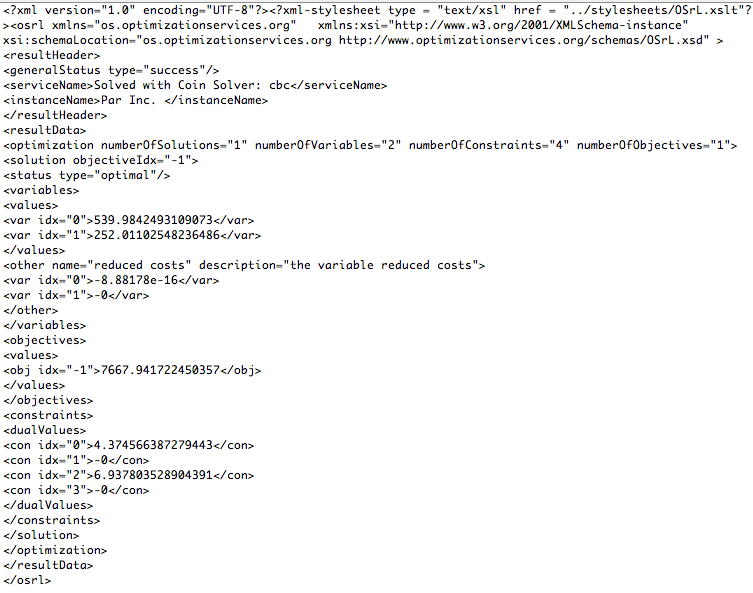
\includegraphics[scale=0.38]{./figures/xmlResult.png}




More detail -- variables values 

\vfill
\begin{verbatim}
<values>
    <var idx="0">539.9842493109073</var>
    <var idx="1">252.01102548236486</var>
</values>\end{verbatim}

\vfill

The objective function value

\vfill

\begin{verbatim}
<objectives>
<values>
<obj idx="-1">7667.941722450357</obj>
</values>
</objectives>
\end{verbatim}



You can also print the result to a file.  

\vfill

Use the osrl option
\vfill

{\small
\begin{verbatim}
OSSolverService -osil ../../data/osilFiles/parincLinear.osil 
    -osrl result.xml
\end{verbatim}
}

\vfill
You can display the result in a browser using XSLT.

\vfill

Copy {\bf data/stylesheets} into the root of the CoinAll distribution. 

\vfill
Open in your browser






To solve a {\bf linear program} set the solver options to:

\begin{itemize}
\vfill \item clp

\vfill \item dylp
\end{itemize}


To solve a {\bf mixed-integer linear program} set the solver options to:

\begin{itemize}
\vfill \item cbc

\vfill \item symphony
\end{itemize}


To solve a {\bf continuous nonlinear program} set the solver options to:

\begin{itemize}
\vfill \item ipopt
\end{itemize}


To solve a {\bf mixed-integer nonlinear program} set the solver options to:

\begin{itemize}
\vfill \item bonmin
\end{itemize}


Solving a {\bf linear integer} program:



\vfill

{\small
\begin{verbatim}
OSSolverService -osil ../../data/osilFiles/p0033.osil 
      -solver cbc
\end{verbatim}
}

\vfill

Solving a {\bf nonlinear} optimization problem

{\small
\begin{verbatim}
OSSolverService -osil ../../data/osilFiles/rosenbrockmod.osil 
      -solver ipopt
\end{verbatim}
}

\vfill

Solving a {\bf mixed-integer nonlinear} optimization problem

{\small
\begin{verbatim}
OSSolverService -osil ../../data/osilFiles/bonminEx1.osil 
      -solver bonmin
\end{verbatim}
}



It is possible to build the OSSolverService to work with other solvers but they are not included due to licensing issues.


\begin{itemize}

\vfill \item Glpk 

\vfill \item Cplex 

\vfill \item LINDO

\end{itemize}




Continually writing out command line options a pain. Use a {\tt configuration} file instead.
Do something like:

\vfill

OSSolverService -config  ../../data/configFiles/testLocal.config

\vfill
where the file {\tt testLocal.config} is

\vfill

\begin{verbatim}
-osil ../../data/osilFiles/parincLinear.osil
-solver cbc
\end{verbatim}

\vfill
{\bf Note:} the only option that is required is the location of an instance file



Finally -- you can call solvers remotely.

\vfill

Specify a {\bf service  location} of the remote solver service.
\vfill

\begin{verbatim}
OSSolverService -osil ../data/osilFiles/parincLinear.osil
  -serviceLocation 
     http://gsbkip.chicagogsb.edu/os/OSSolverService.jws
\end{verbatim}











To get help

\vfill
\begin{verbatim}
OSSolverService -h     
\end{verbatim}

 --OR--    
 
\begin{verbatim} 
OSSolverService --help
\end{verbatim}






See also for calling remote solvers. 

\section{Calling COIN-OR  Solvers using a Modeling Language}

Mention GAMSlinks

\section{Using Visual Studio to Build Application}

\section{Example Projects}


\end{document}